%%%%%%%%%%%%%%%%%%%%%%%%%%%%%%%%%%%%%%%%%%%%%%%%%%%%%%%%%%%%%%%%%%%%%%%%%%
% SwitchOnBehaviorAndSwitchOffBehaviorOfUI
%%%%%%%%%%%%%%%%%%%%%%%%%%%%%%%%%%%%%%%%%%%%%%%%%%%%%%%%%%%%%%%%%%%%%%%%%%

\begin{figure}[htb]
    \centering
    \begin{minipage}[t]{0.45\textwidth}
        \centering
        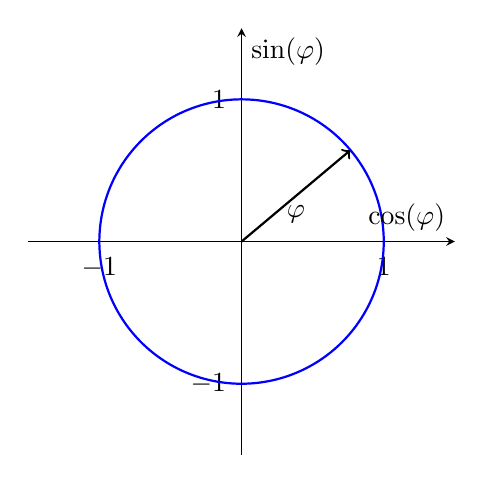
\begin{tikzpicture}
            \begin{axis}[
                axis lines=middle, 
                xlabel={$\cos(\varphi)$},
                ylabel={$\sin(\varphi)$},
                width=7cm, height=7cm,
                major grid style={line width=.2pt,draw=gray!50},
                minor grid style={line width=.1pt,draw=gray!20},
                xmin=-1.5, xmax=1.5,
                ymin=-1.5, ymax=1.5,
              ]
              
              \draw[thick, ->] (0,0) -- ({cos(40)}, {sin(40)}) node[above right] {};
              \node at ({0.5*cos(40)}, {0.5*sin(40)}) [below] {$\varphi$};

              \addplot[
                  domain=0:360, 
                  samples=200,  
                  thick,
                  color=blue,
              ]
              ({cos(x)}, {sin(x)}); 
            \end{axis}
        \end{tikzpicture}
    \end{minipage}
    \hspace{0.5cm}
    \begin{minipage}[t]{0.45\textwidth}
        \centering
        \begin{tikzpicture}
            \draw[->] (-2,0) -- (2,0) node[right] {}; 
            \draw[->] (0,-2) -- (0,2) node[above] {}; 
            \node at (-1.5,1.5) {$\cos\left(k \frac{\pi}{2}\right)$};
            \node at (-2,0) [left] {$2,6,\ldots$}; 
            \node at (2,0) [right] {$0,4,\ldots$}; 
            \node at (0,2) [above] {$1,5,9,13,\ldots$}; 
            \node at (0,-2) [below] {$3,7,11,15,\ldots$}; 

            % Kreuz bei jedem markierten Punkt
            \foreach \x/\y in {-1.5/0, 1.5/0, 0/1.5, 0/-1.5} {
                \draw[thick]
                    (\x,\y) +(-0.1,0.1) -- +(0.1,-0.1) % Diagonale des Kreuzes
                             +(-0.1,-0.1) -- +(0.1,0.1); % Andere Diagonale des Kreuzes
            }
        \end{tikzpicture}
    \end{minipage}
        
    \begin{tikzpicture}
        \draw[->] (-2,0) -- (2,0) node[right] {}; 
        \draw[->] (0,-2) -- (0,2) node[above] {}; 
        \node at (-1.5,1.5) {$\cos\left(k \frac{\pi}{3}\right)$};
        \node at (-2,0) [left] {$2,6,\ldots$}; 
        \node at (2,0) [right] {$0,4,\ldots$}; 
        \node at (0,2) [above] {$1,5,9,13,\ldots$}; 
        \node at (0,-2) [below] {$3,7,11,15,\ldots$}; 

        % Kreuz bei jedem markierten Punkt
        \foreach \x/\y in {-1.5/0, 1.5/0, 0/1.5, 0/-1.5} {
            \draw[thick]
                (\x,\y) +(-0.1,0.1) -- +(0.1,-0.1) % Diagonale des Kreuzes
                         +(-0.1,-0.1) -- +(0.1,0.1); % Andere Diagonale des Kreuzes
        }
    \end{tikzpicture}
    \hspace{1cm} % Abstand zwischen den beiden Diagrammen
    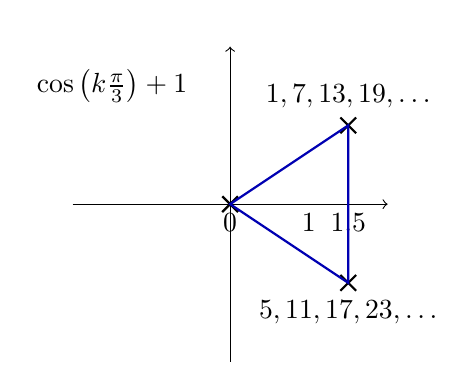
\begin{tikzpicture}
        % Koordinatensystem zeichnen
        \draw[->] (-2,0) -- (2,0) node[right] {}; 
        \draw[->] (0,-2) -- (0,2) node[above] {}; 
        \node at (-1.5,1.5) {$\cos\left(k \frac{\pi}{3}\right)+1$};
    
        % Beschriftungen an der x-Achse
        \foreach \x in {0, 1, 1.5} {
            \node at (\x, 0) [below] {\x};
        }
    
        % Beschriftungen an spezifischen Punkten
        \node at (1.5,1.1) [above] {$1,7,13,19,\ldots$}; 
        \node at (1.5,-1.1) [below] {$5,11,17,23,\ldots$}; 
    
        % Kreuz bei jedem markierten Punkt
        \foreach \x/\y in {0/0, 1.5/1, 1.5/-1} {
            \draw[thick]
                (\x,\y) +(-0.1,0.1) -- +(0.1,-0.1) % Diagonale des Kreuzes
                         +(-0.1,-0.1) -- +(0.1,0.1); % Andere Diagonale des Kreuzes
        }
    
        % Verbindungslinien zwischen den Punkten
        \draw[thick, color=blue!70!black]
            (0,0) -- (1.5,1) -- (1.5,-1) -- cycle;
    \end{tikzpicture}
    \caption{Graphical solution of the cos terms.}
    \label{fig:Graphical solution of the cos terms}
\end{figure}
